%diagrams
\begin{center}
\begin{figure}[h]
	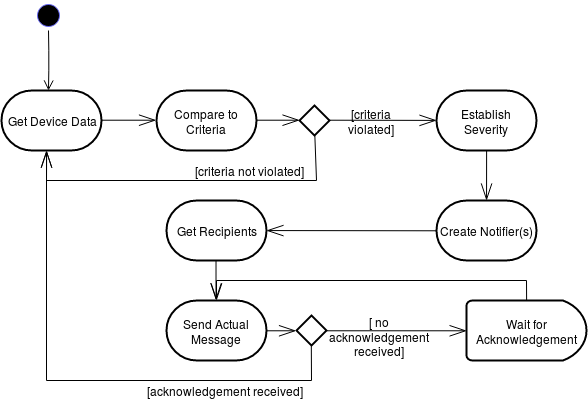
\includegraphics[width=15cm, height=13cm]{Notification/NotificationActivity.png}
\end{figure}
\end{center}

\begin{center}
\begin{figure}[h]
	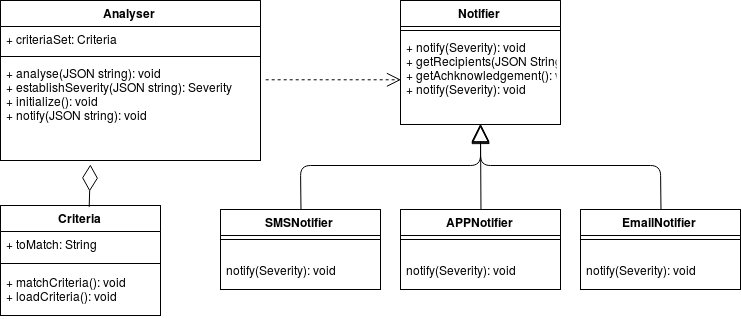
\includegraphics[width=15cm, height=8cm]{Notification/NotificationsClass.png}
\end{figure}
\end{center}

%description
\begin{itemize}
	\item Analyser\\
	The Analyser class is responsible for getting the data from the real time stream and comparing the data to specific criteria. It serves as the "Subject." It also establishes the severity of a violation of criteria and takes anomalities into account. This means that if the device is plugged out and then in again, the severity will not be as bad as when a heart rate steadily decreases over time. 	
	
	\item Criteria\\
	The criteria are device-specific and are stored inside the database proir to runtime. Each Criteria object have a function that matches the input data to a specific criteria and returns a boolean that says wheather the criteria was violated or not. These objects are the "Oservers."
	
	\item Notifier\\
	In the case of a violation, a Notifier class is created. It gets the appropriate subscriber list, or recipient list, from the database, and sends the actual notification to the recipient(s). The Notifier class	itself is only an abstract class that houses the main functionality.
	
	\item SMSNotifier, APPNotifier, EmailNotifier\\
	These three are the concrete implementations of the Notifier class.
\end{itemize}

%design patterns
The main design pattern used for this event-driven system is Observer. Analyser is the Subject that houses the data being observed. The actual observations are done by the Criteria objects. 

Another design pattern used is the Template Method. Notifier serves as the abstract class that has all the main algorithms and provides the interface functions. SMSNotifier, APPNotifier, and EmailNotifier are the concrete classes which implement the Notifier class's notify() function.